
\Problem{Triangles de Sierpiński}

\Statement

El triangle de Sierpiński és un objecte fractal, que va ser introduït per primera vegada en 1915
pel matemàtic polonès Waclaw Sierpiński. És un dels exemples bàsics de conjunt auto-semblant,
una de les propietats fonamentals de les fractals.

\medskip

Per pintar un triangle de Sierpiński de mida $m$ amb un sol nivell, cal pintar
un triangle equilàter de costat $m$. Per pintar un triangle de Sierpiński de mida
$m$ i $n\ge2$ nivells, cal pintar tres subtriangles de Sierpiński de mida $m/2$ amb $n-1$ nivells.
El segon triangle s'ha de pintar a la dreta del vèrtex dret del primer, el tercer s'ha de pintar
al damunt del vèrtex superior del primer.

\bigskip

Per exemple, aquests són triangles de Sierpiński amb 1, 2, 3, 4, 5 i 6 nivells:

\begin{center}
1 ~
\fbox{
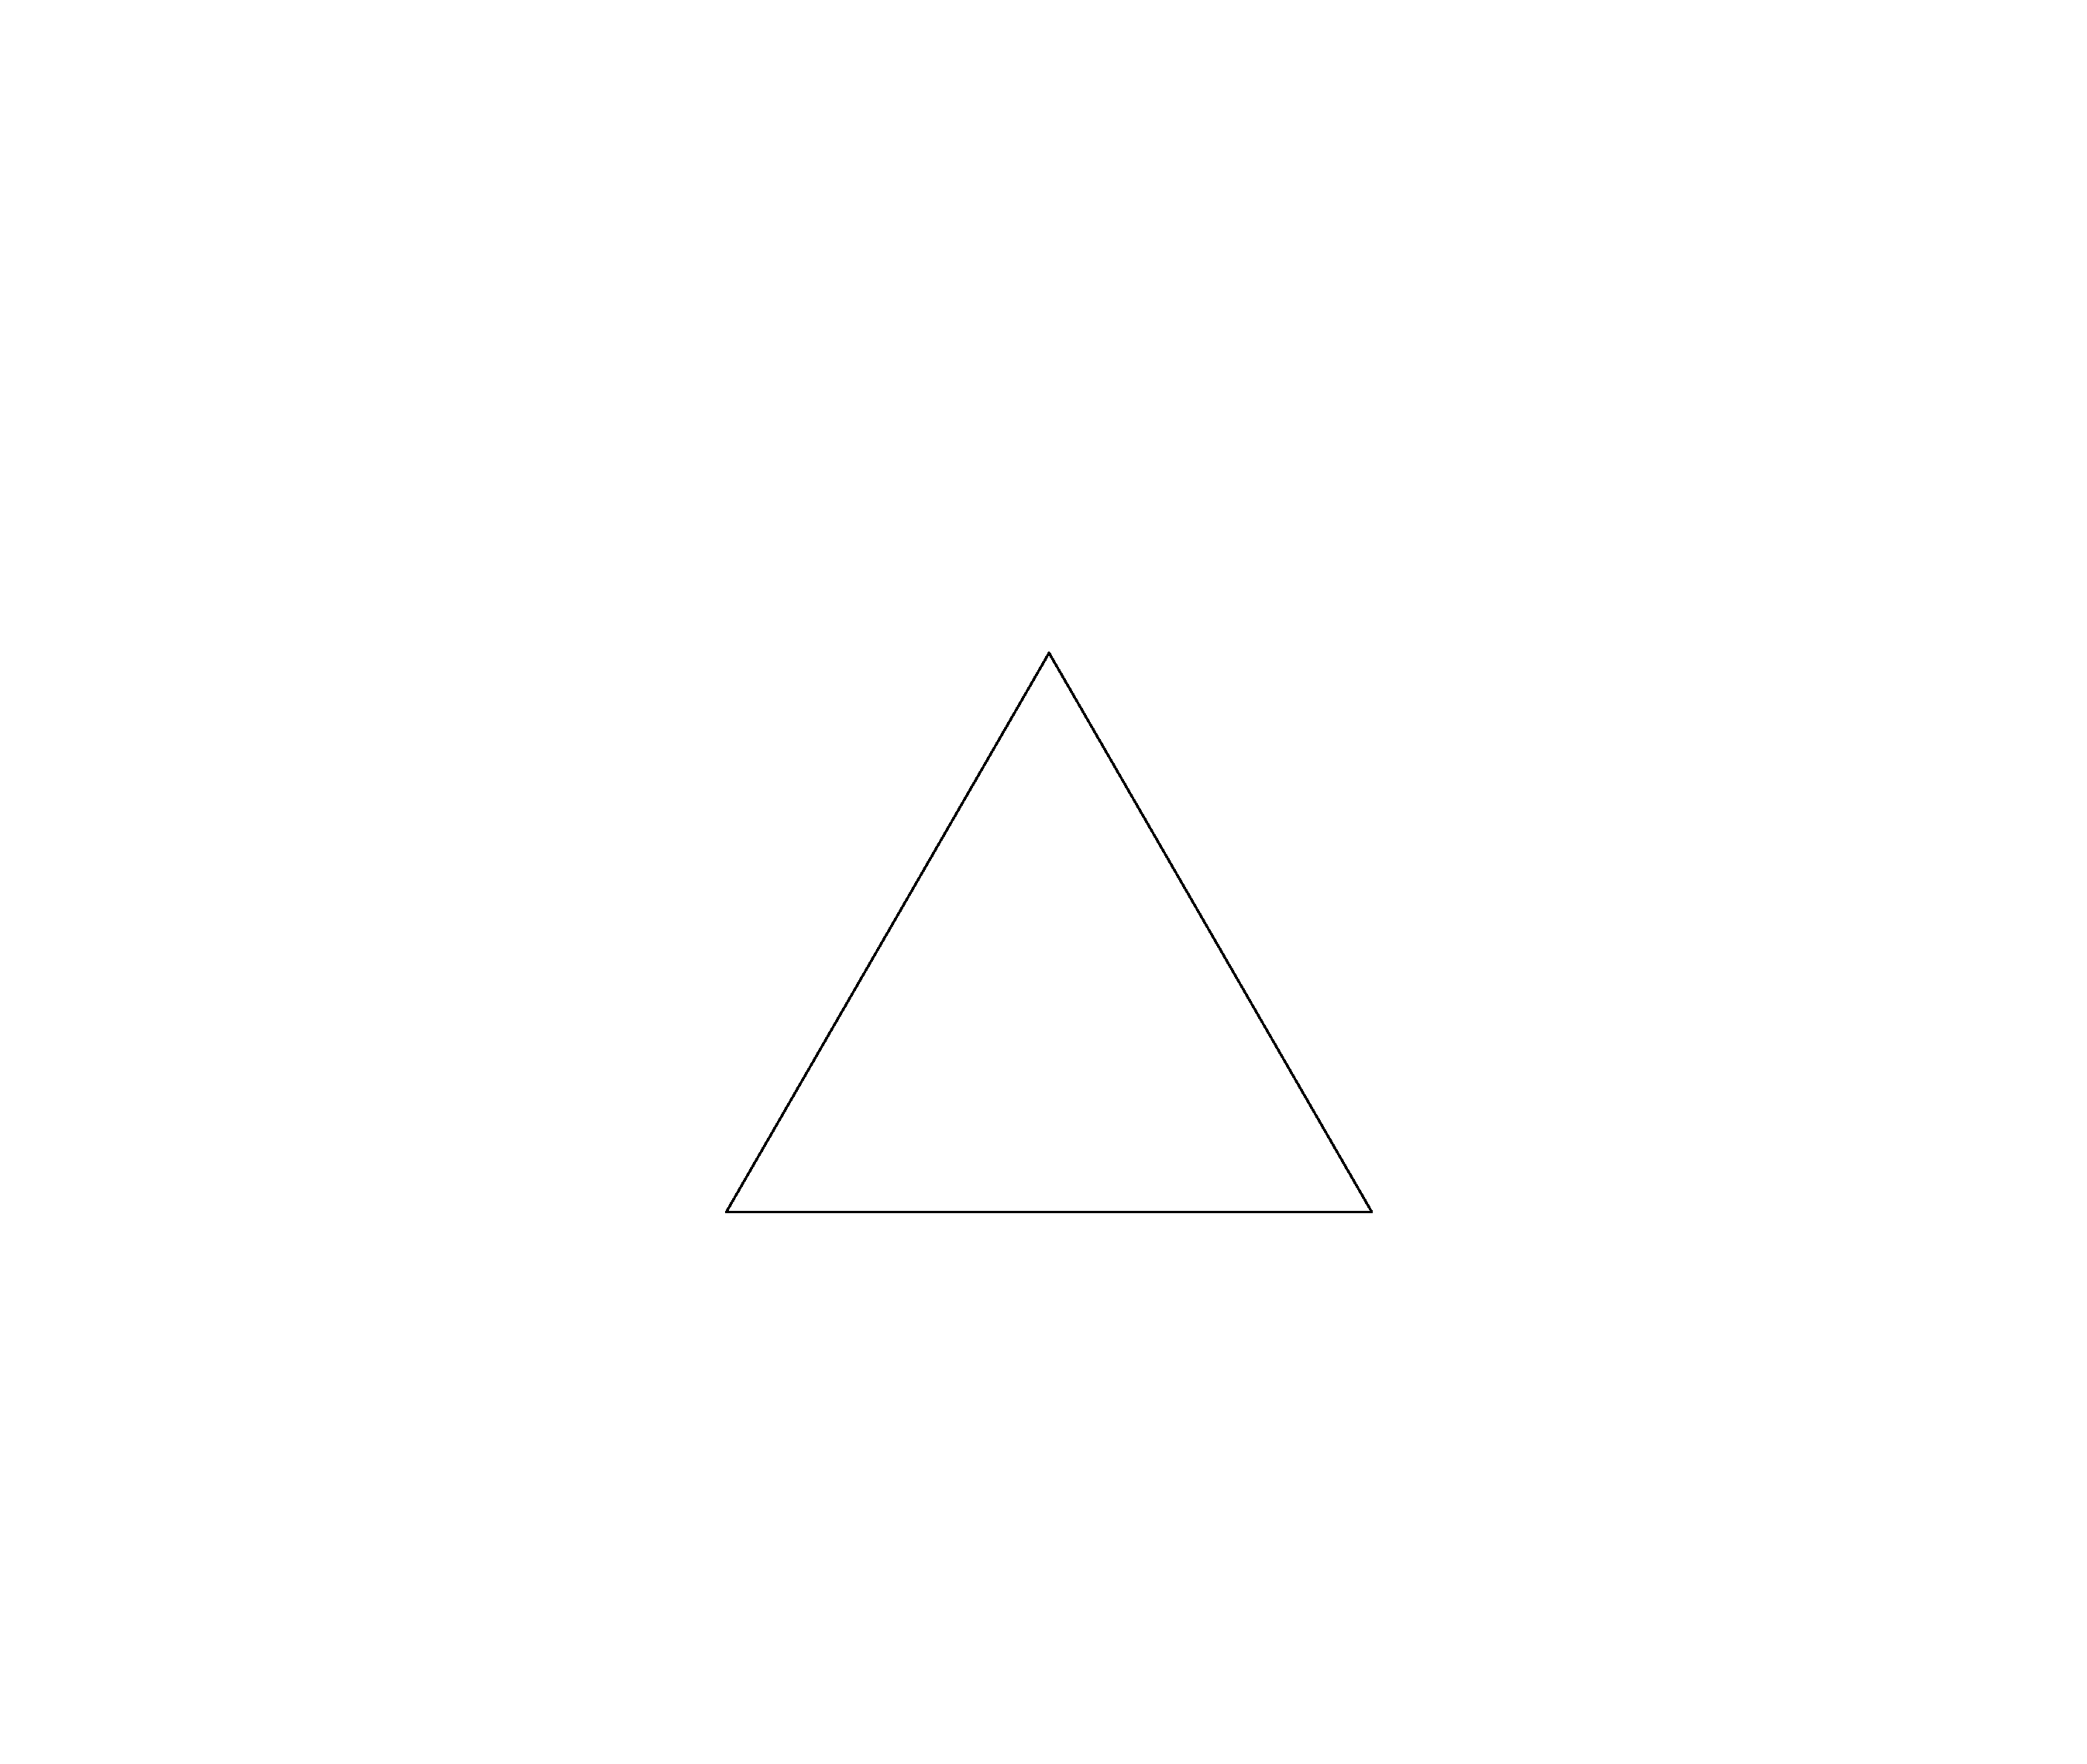
\includegraphics[trim=450 300 450 375,height=3.5cm]{1.eps}
}
\qquad
2 ~
\fbox{
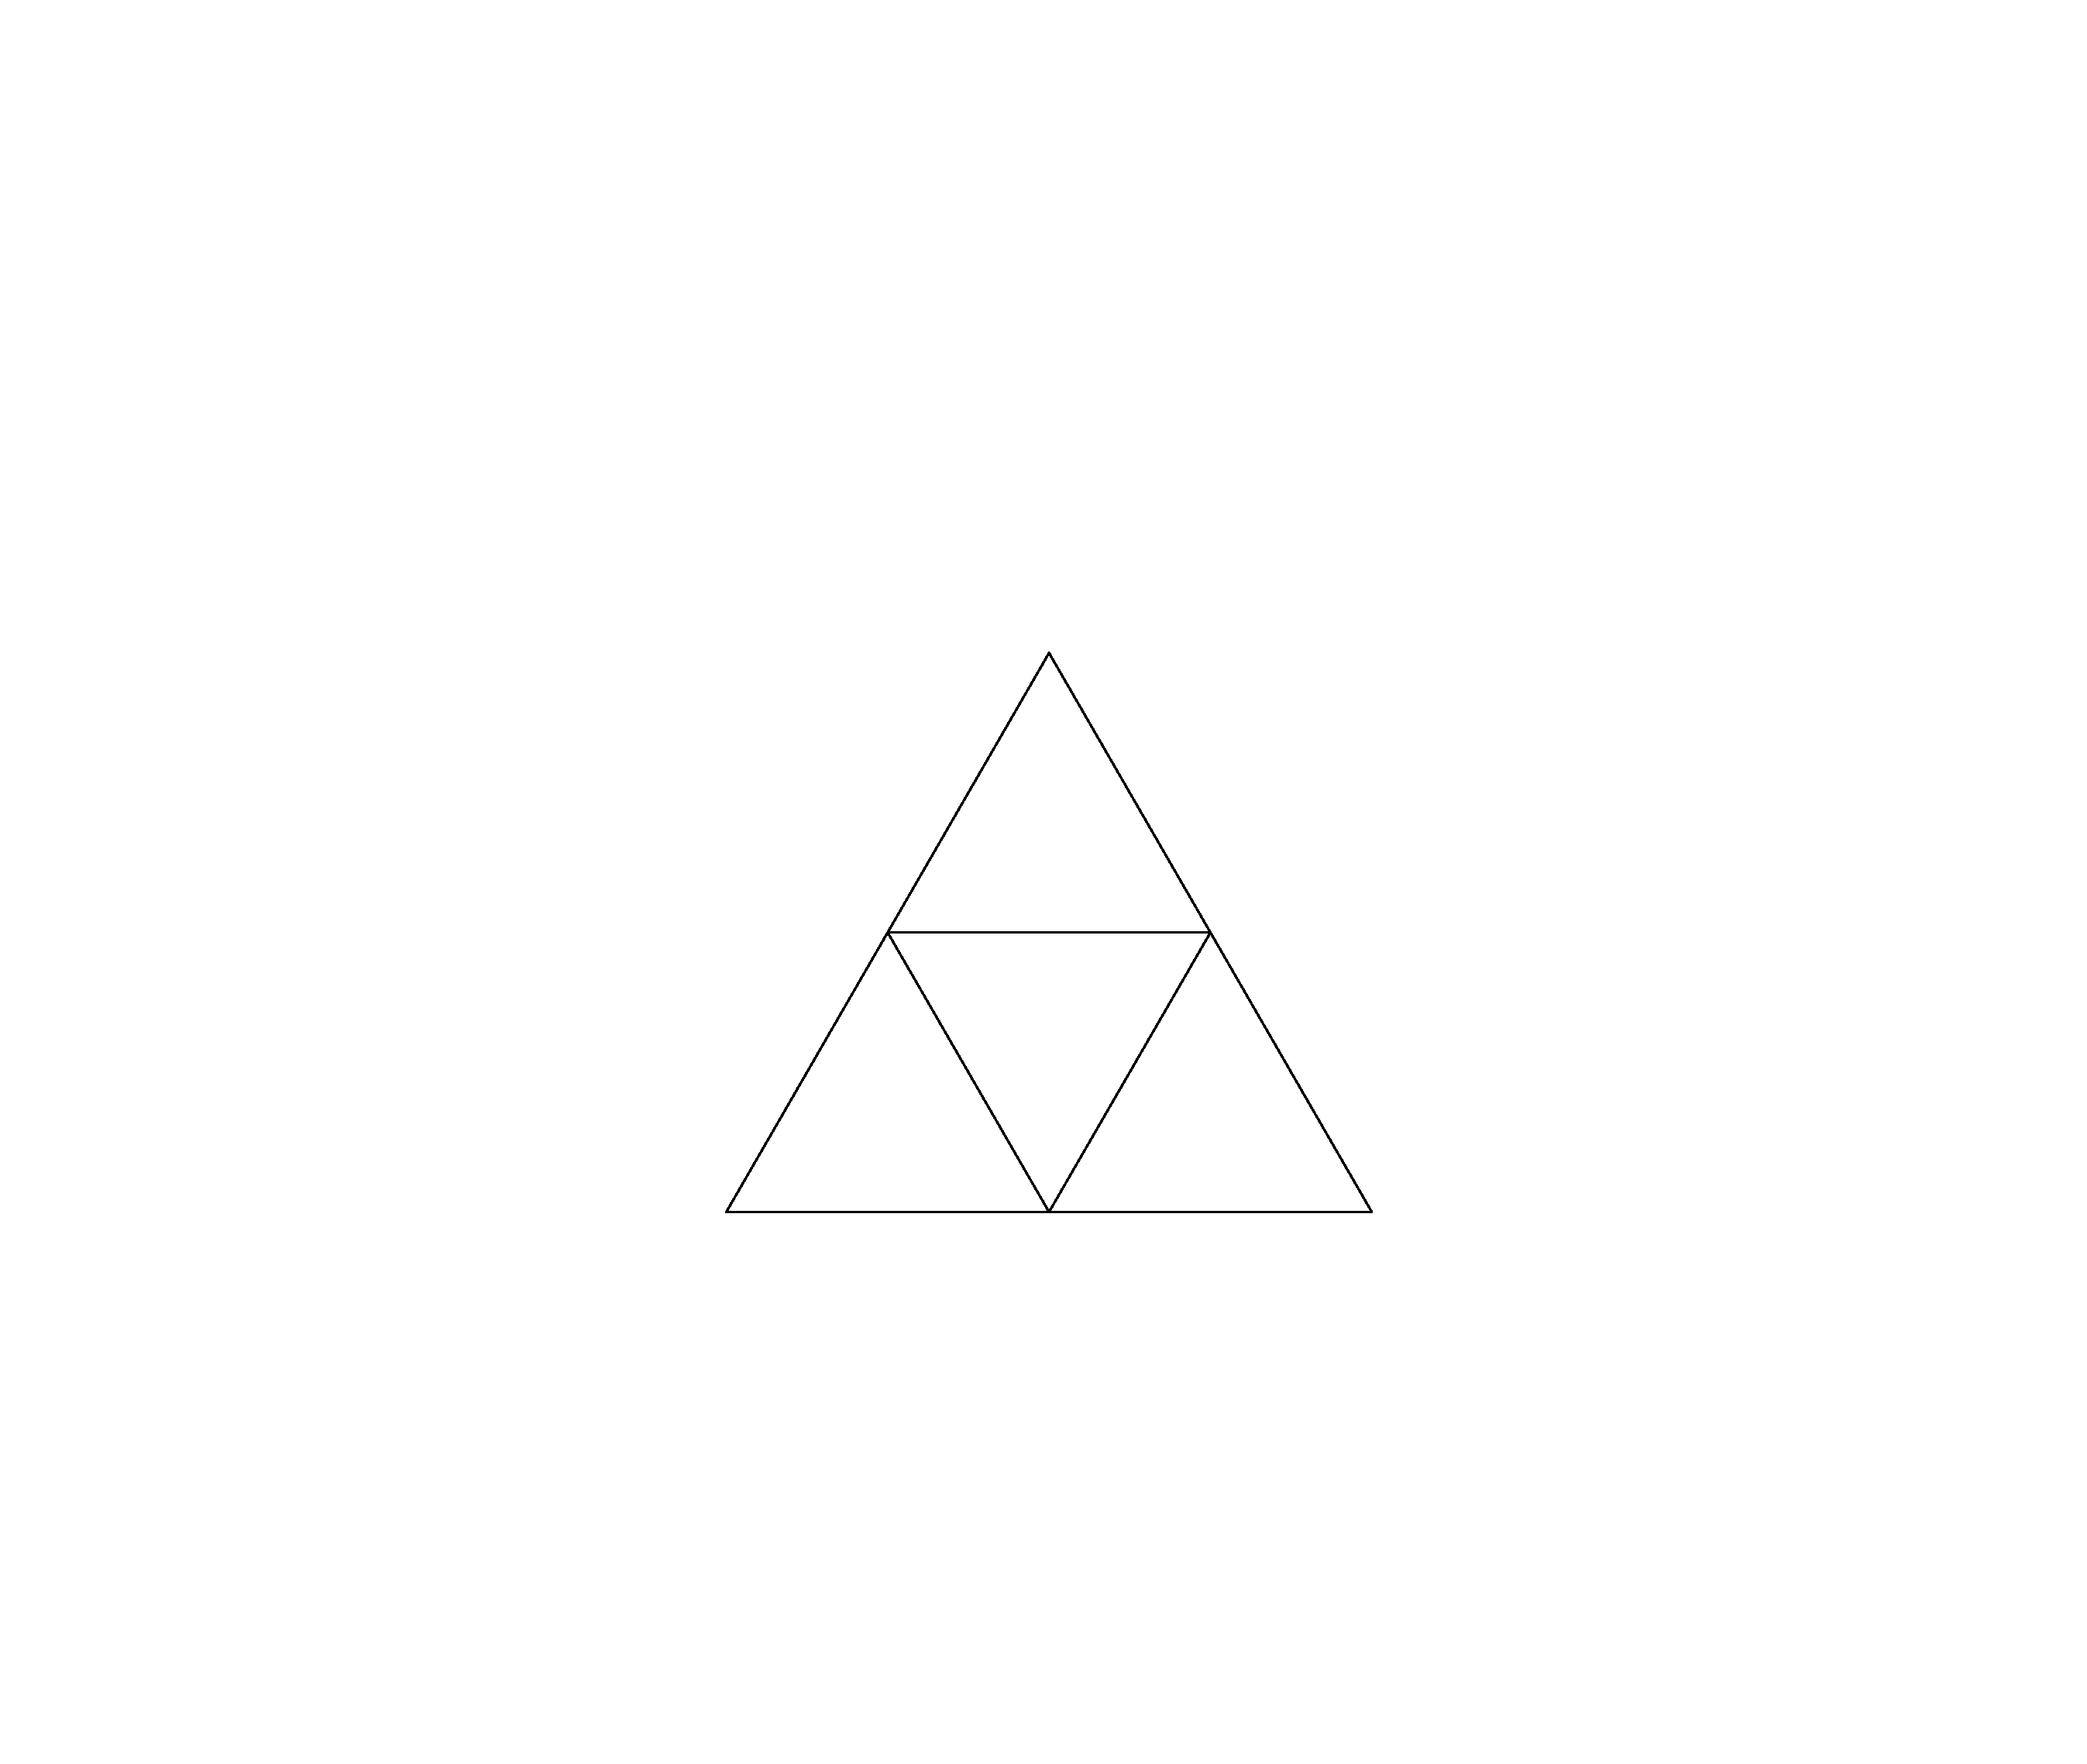
\includegraphics[trim=450 300 450 375,height=3.5cm]{2.eps}
}
\qquad
3 ~
\fbox{
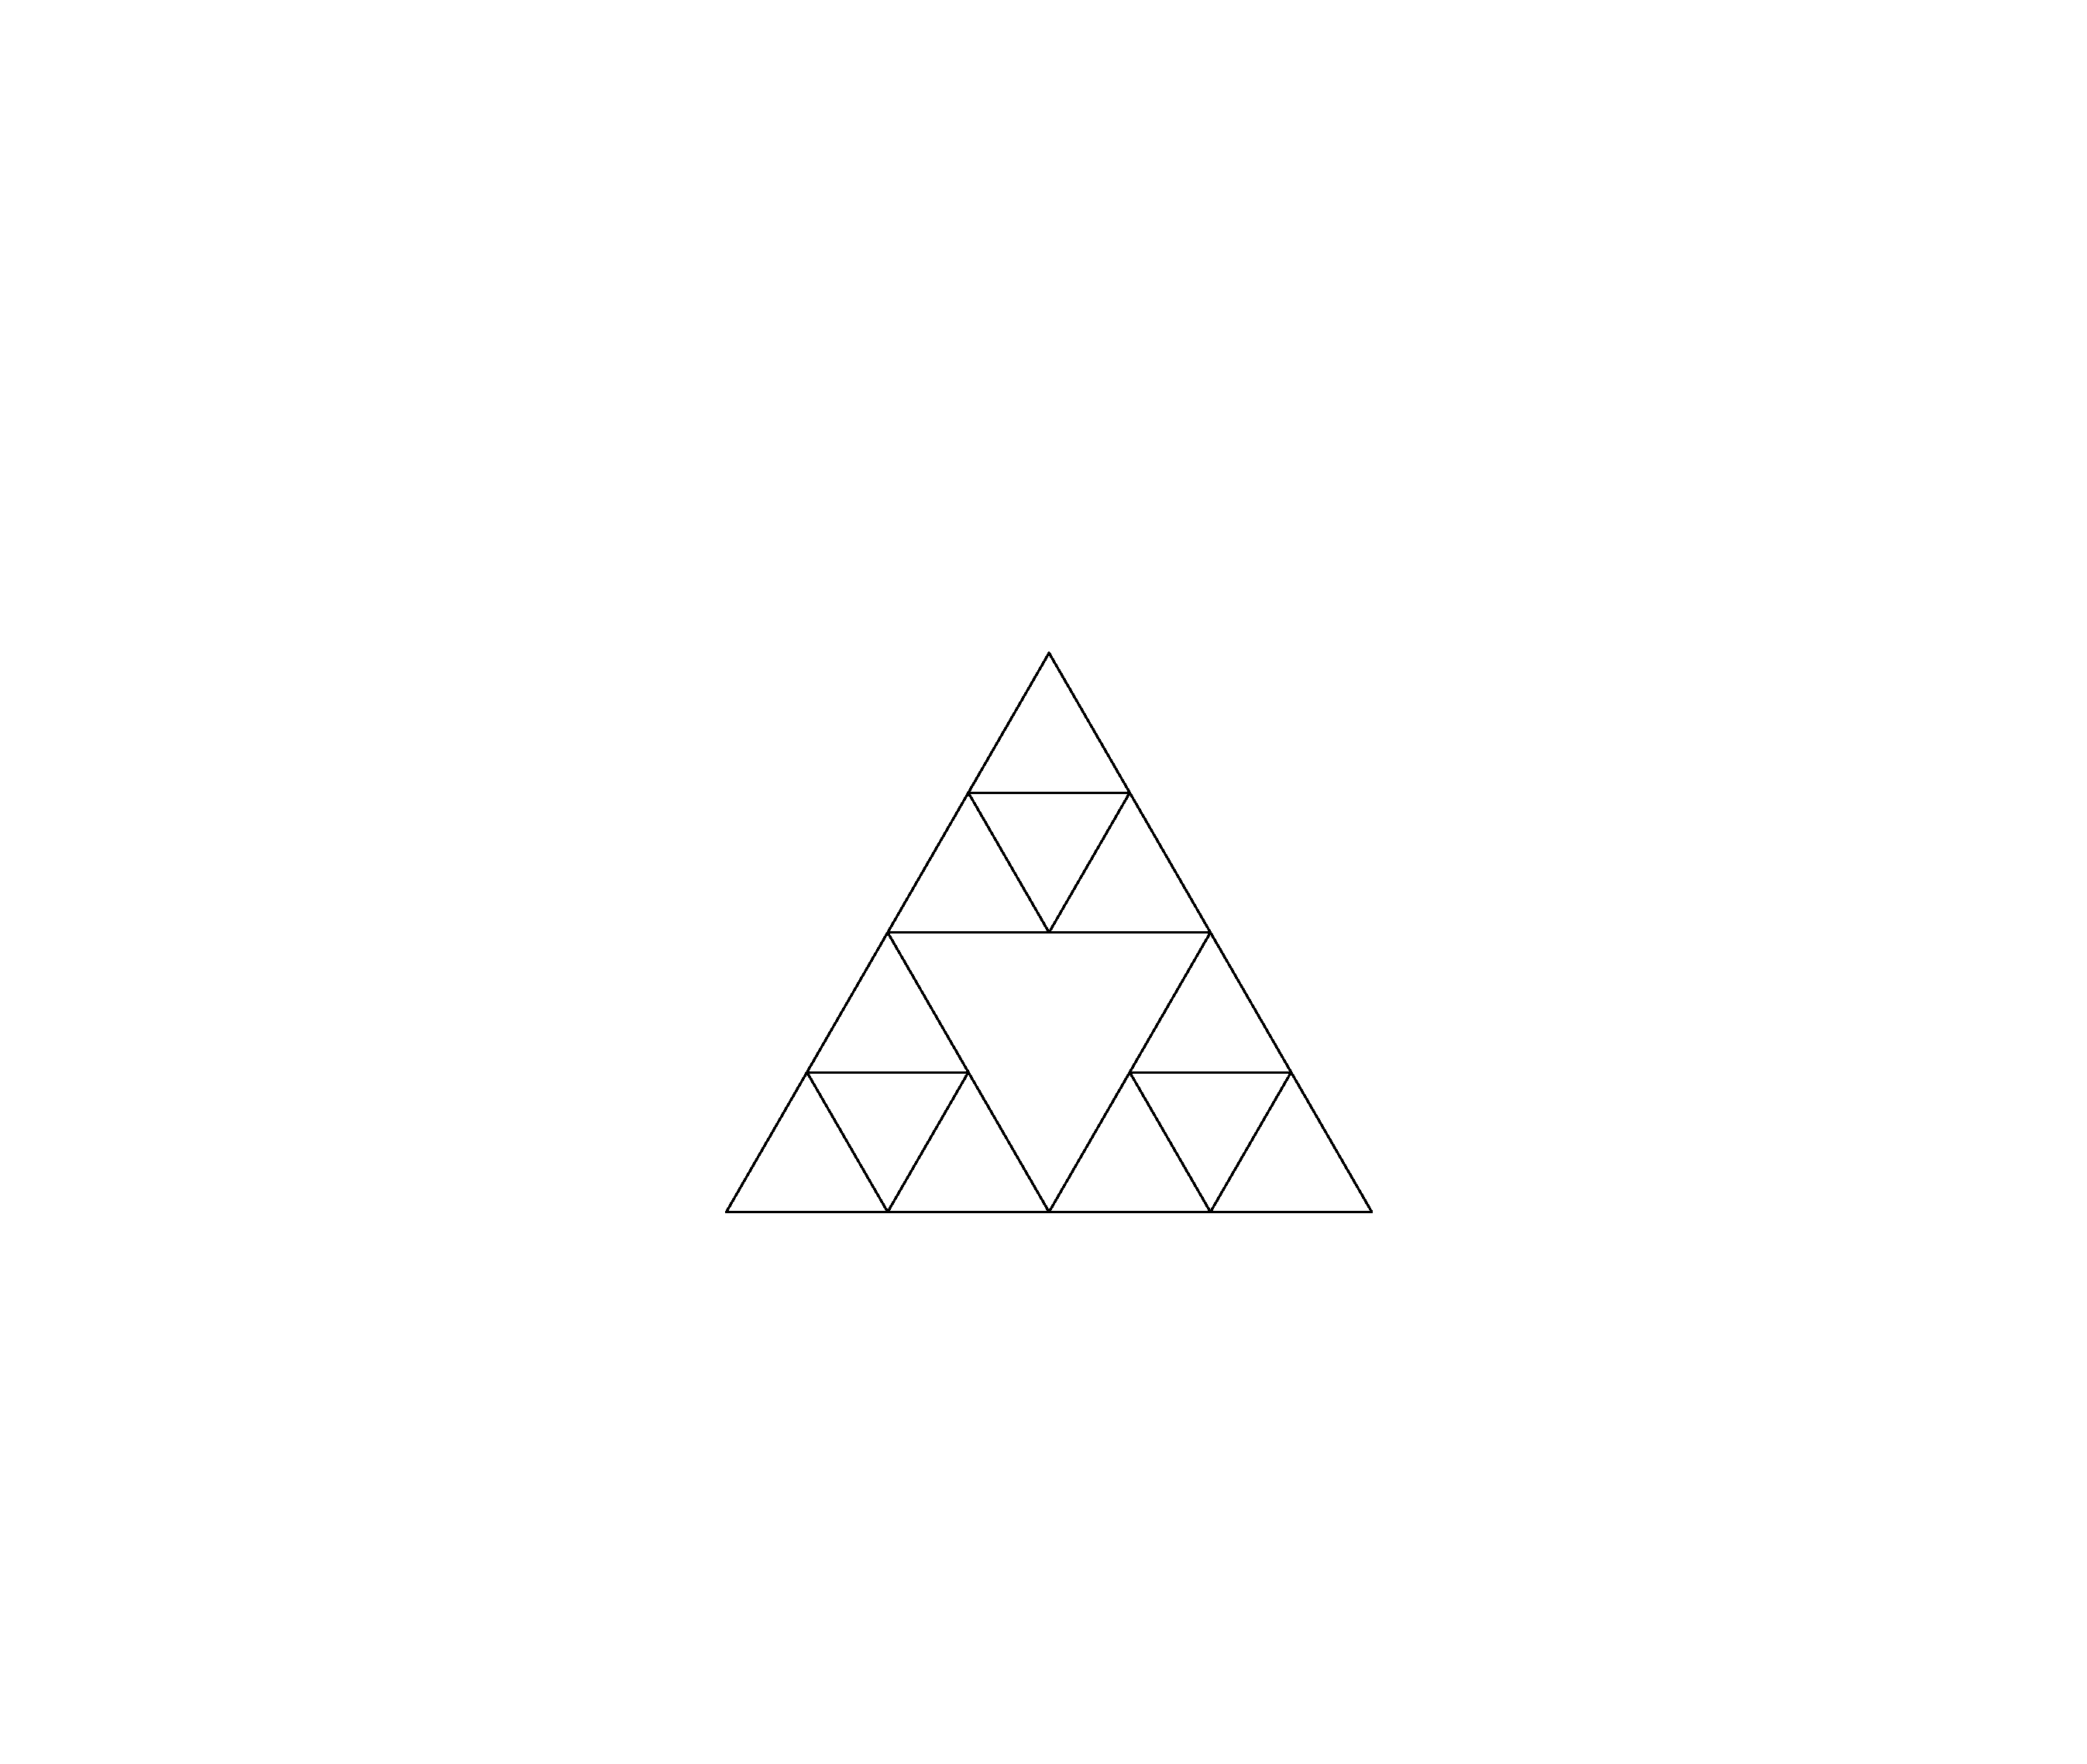
\includegraphics[trim=450 300 450 375,height=3.5cm]{3.eps}
}

\bigskip
\bigskip

4 ~
\fbox{
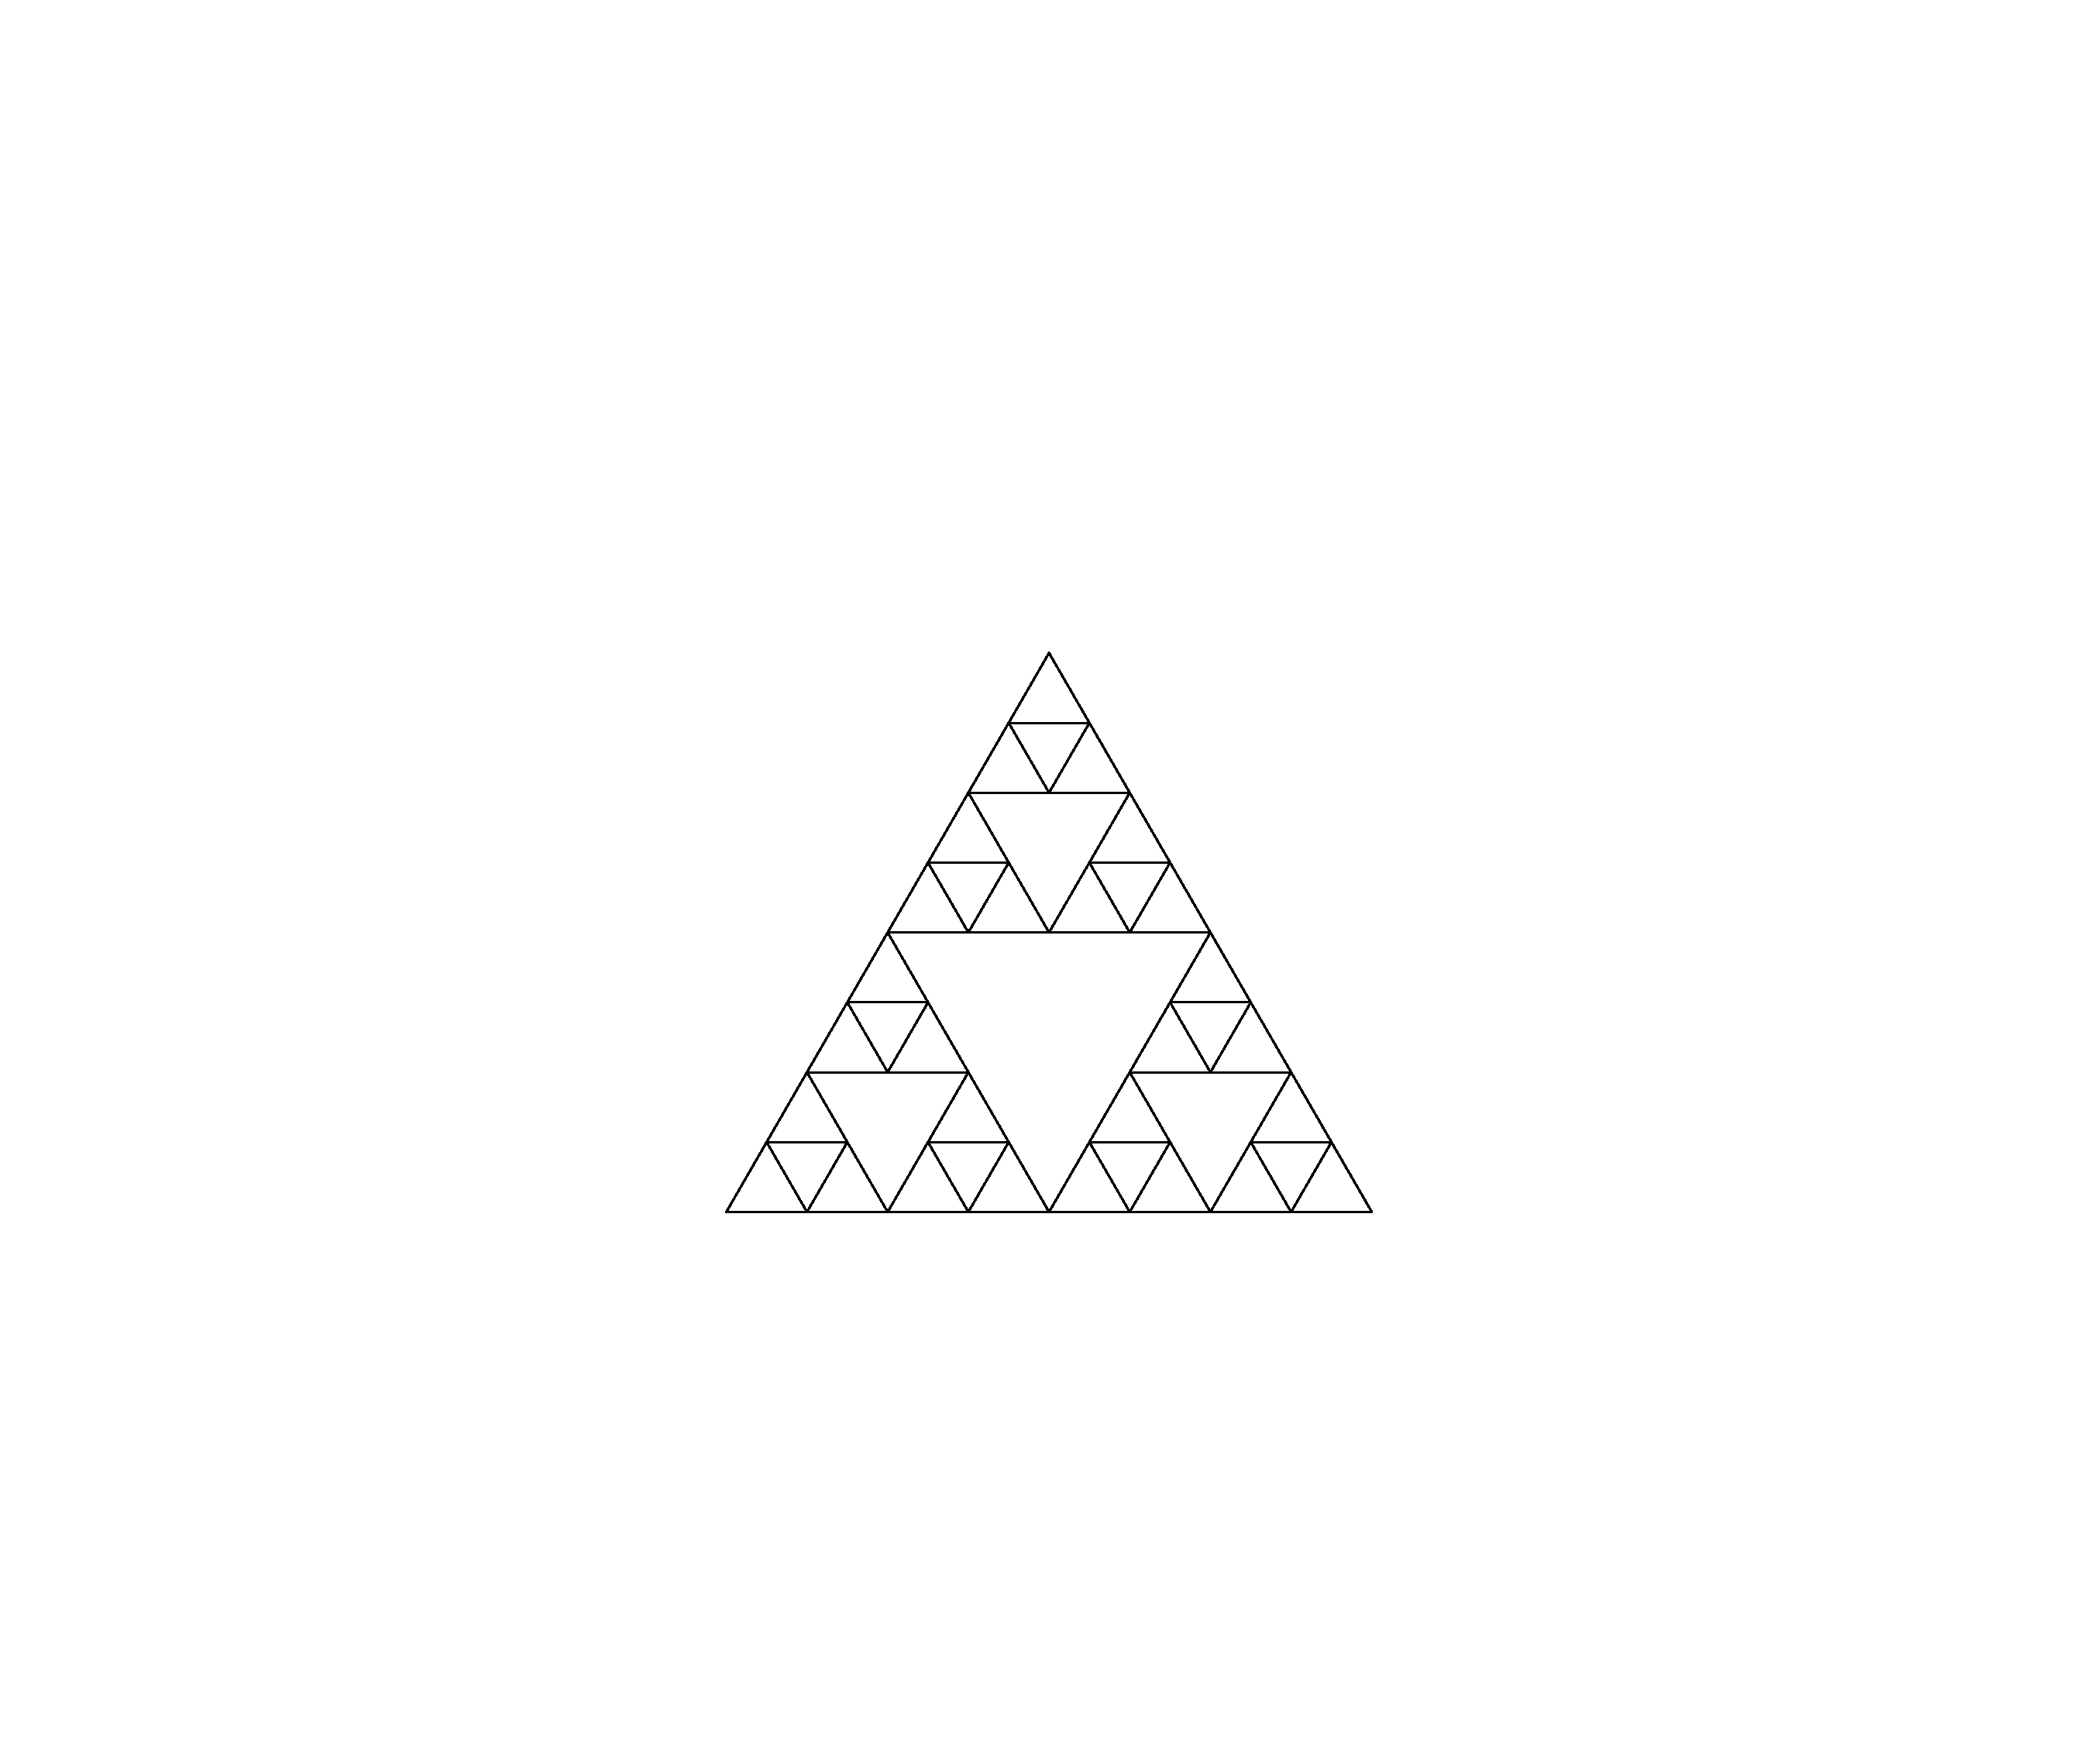
\includegraphics[trim=450 300 450 375,height=3.5cm]{4.eps}
}
\qquad
5 ~
\fbox{
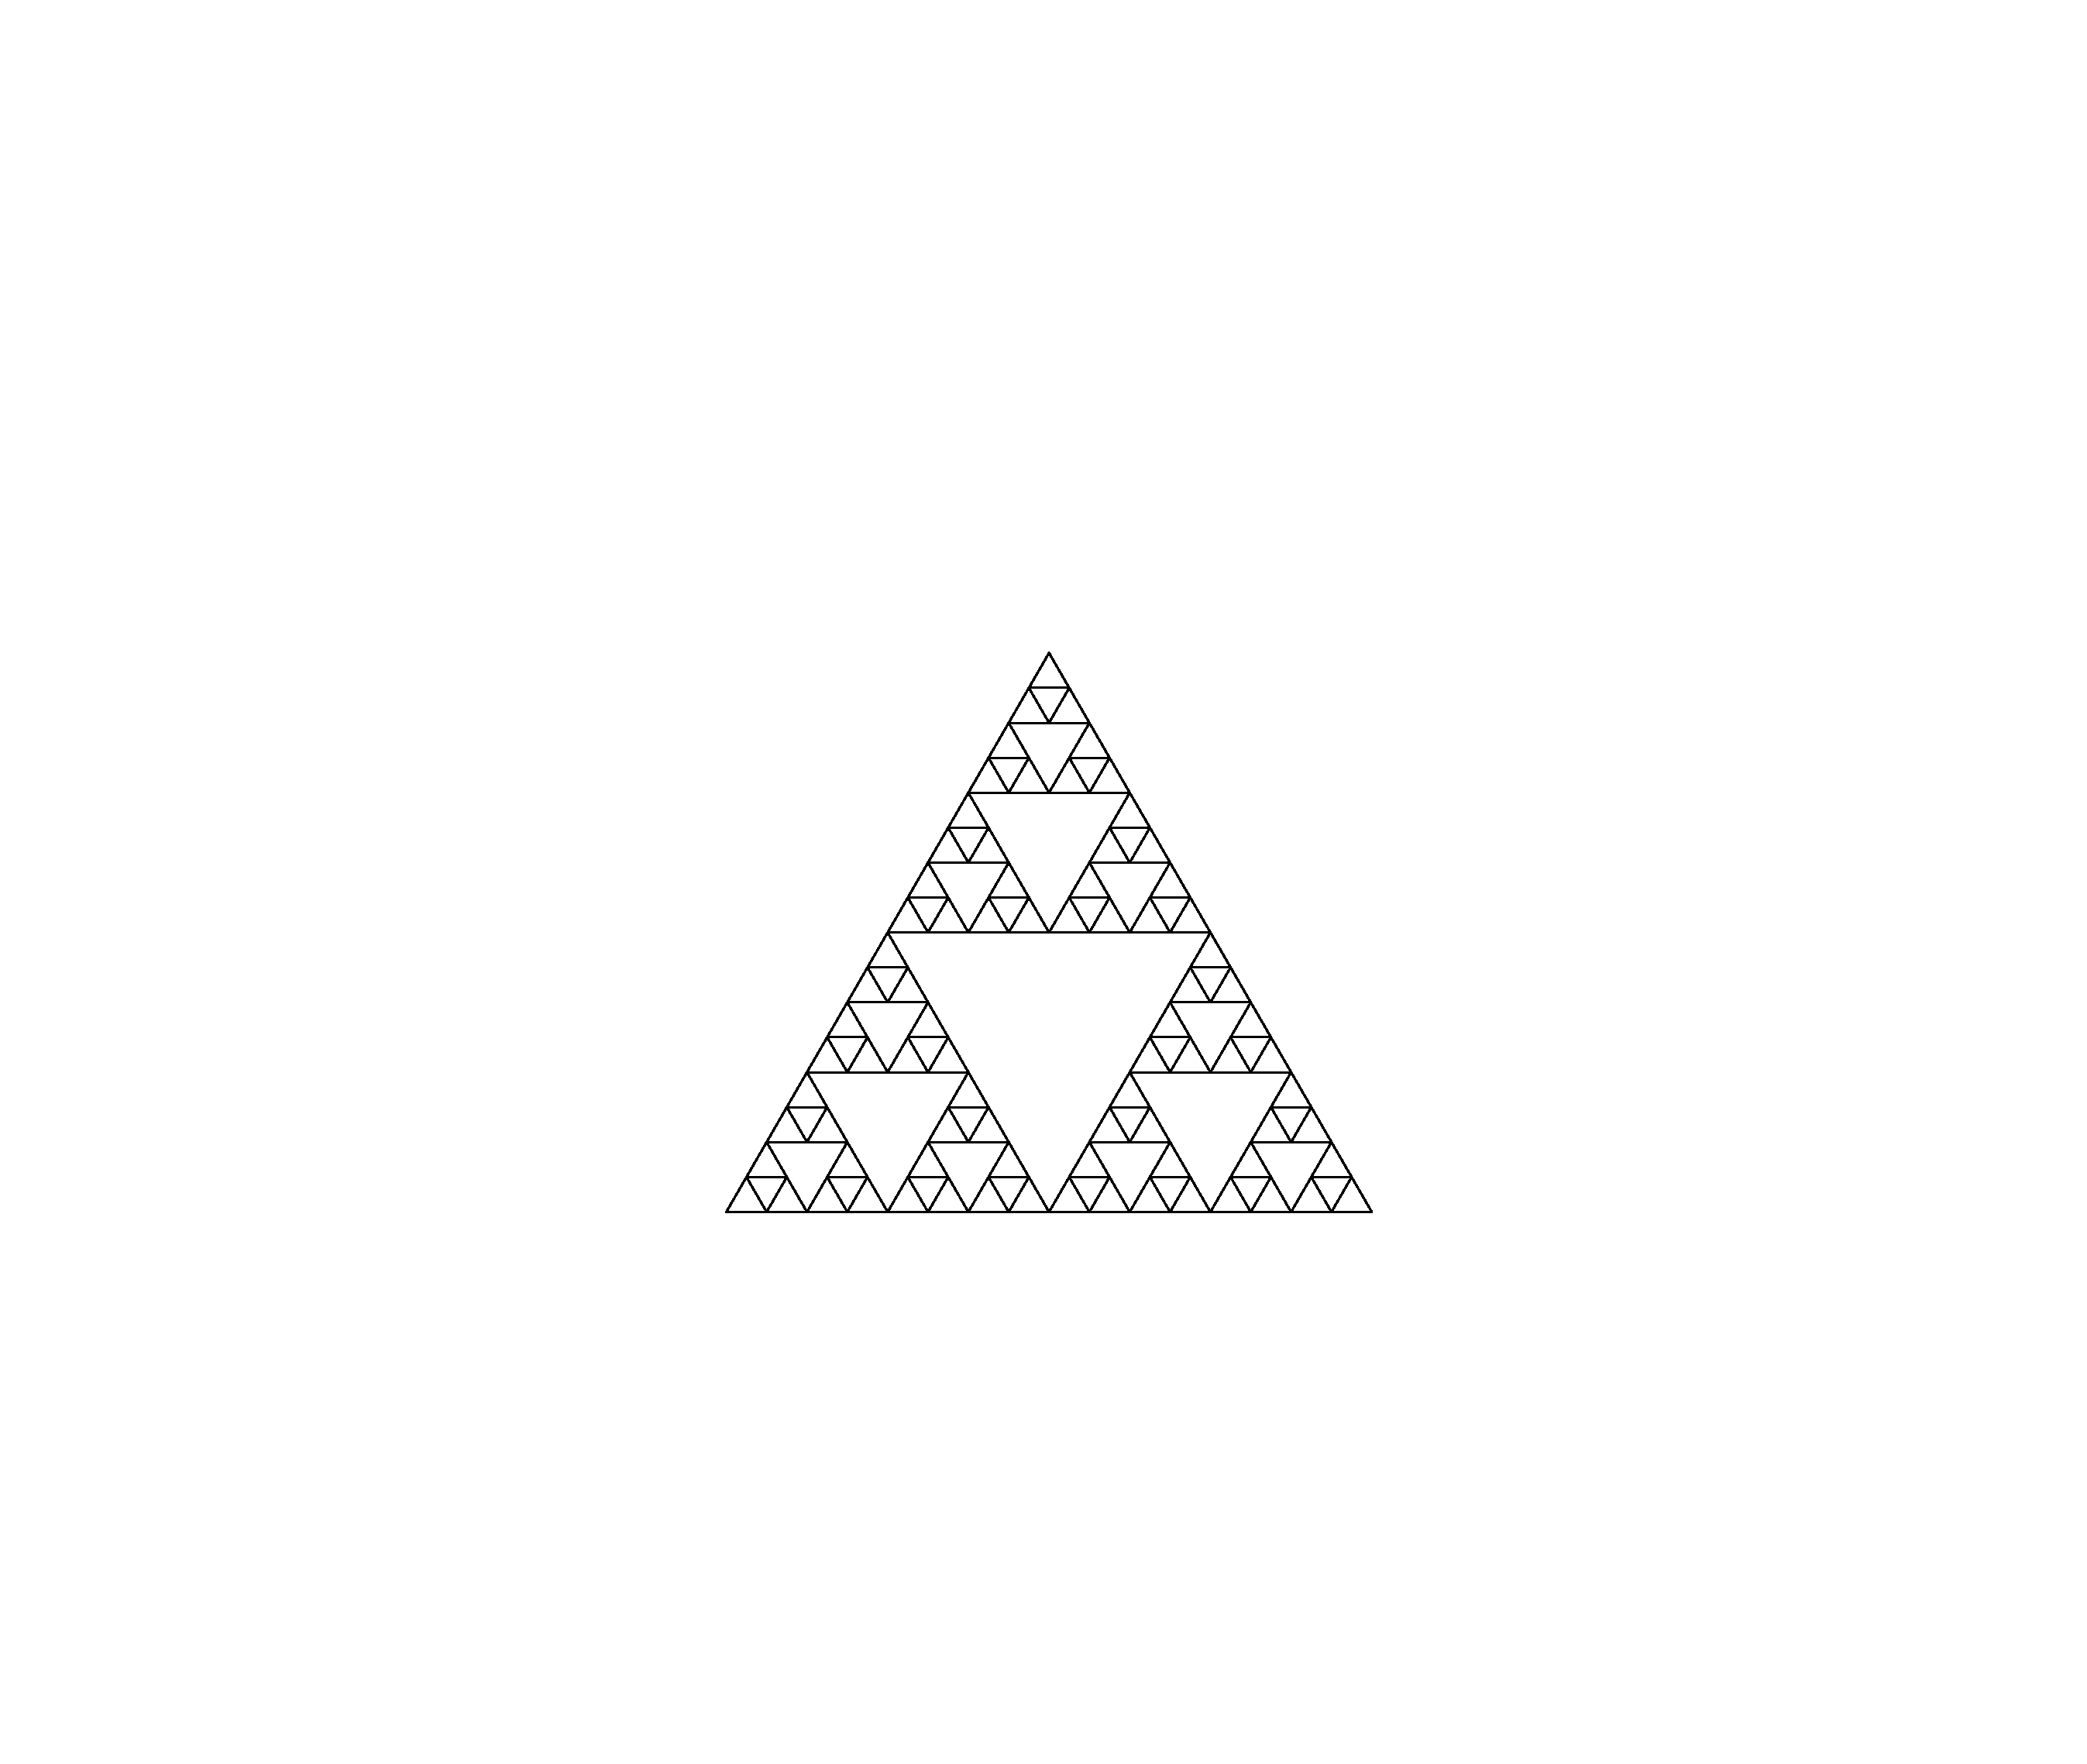
\includegraphics[trim=450 300 450 375,height=3.5cm]{5.eps}
}
\qquad
6 ~
\fbox{
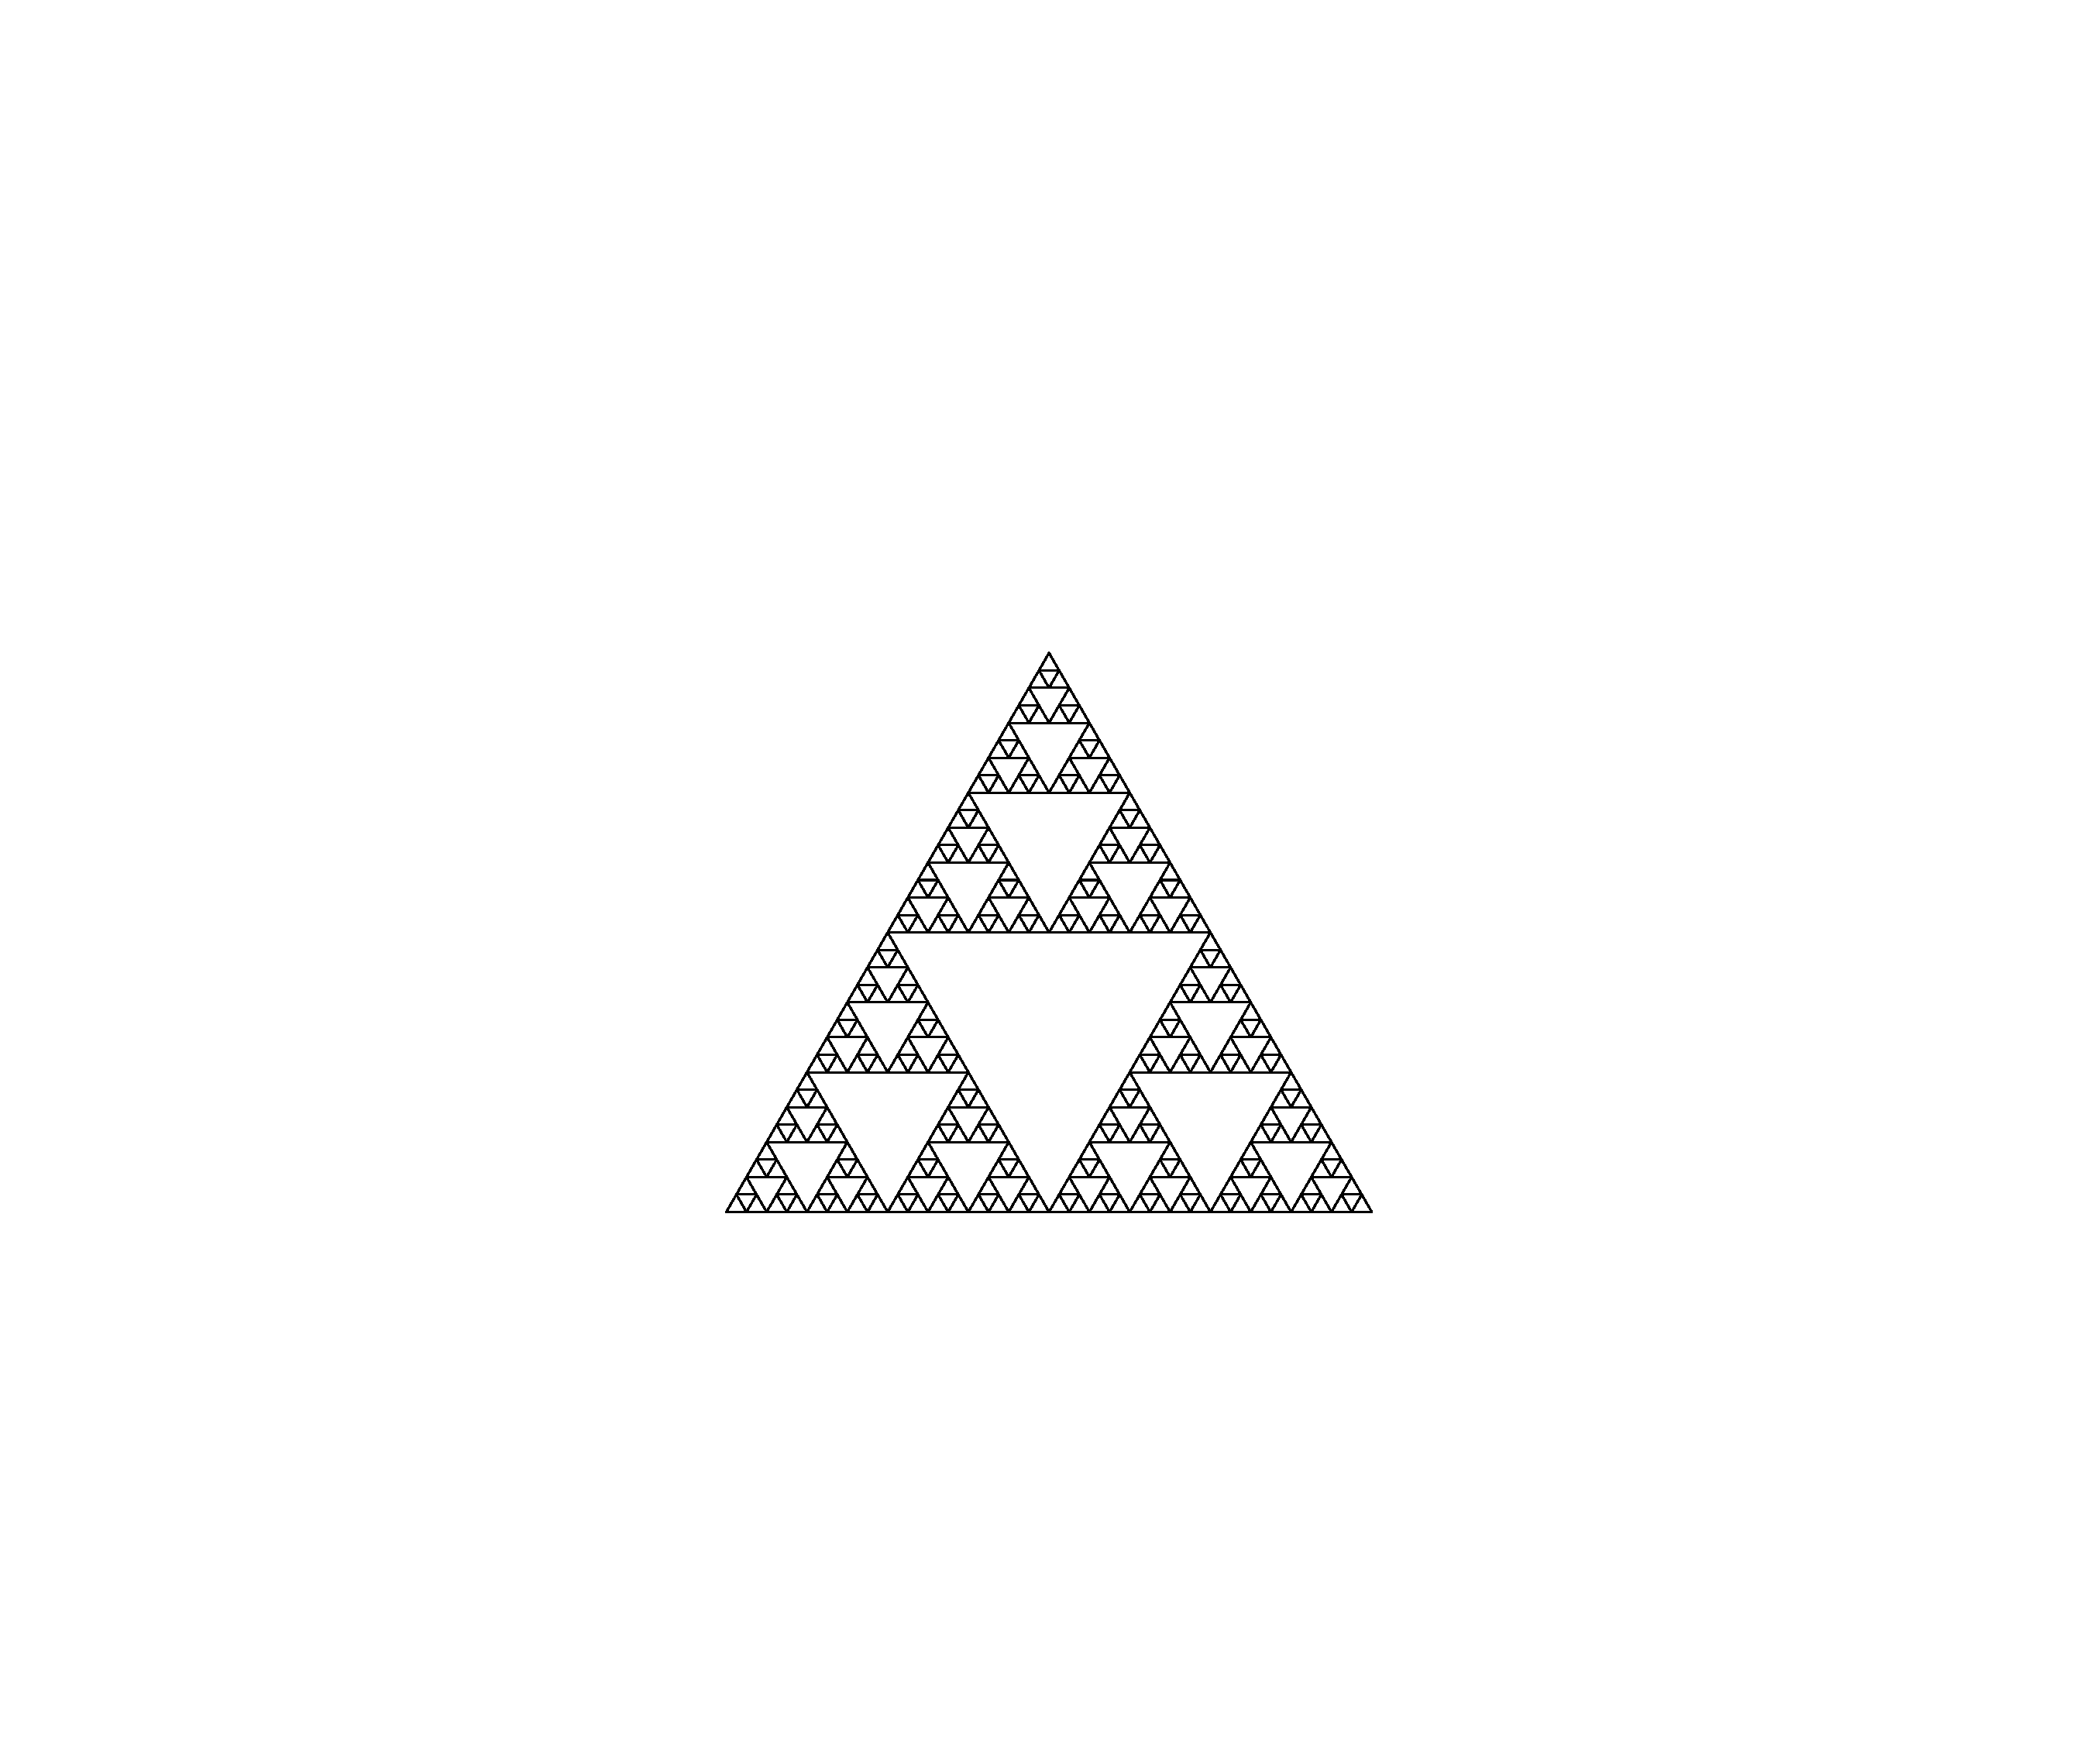
\includegraphics[trim=450 300 450 375,height=3.5cm]{6.eps}
}
\end{center}

\mysection{Entrada}

A l'entrada, es dónen dos valors:
un real positiu $m$ amb la mida del triangle de Sierpiński, i
un natural $n$ amb el seu nombre de nivells.

\mysection{Sortida}

El programa ha de dibuixar un triangle de Sierpiński de mida $m$ amb $n$ nivells.

\clearpage

\begin{multicols}{2}\raggedcolumns
\mysection{Exemple d'entrada 1}

\begin{verbatim}
100
2
\end{verbatim}

\columnbreak

\mysection{Exemple de sortida 1}

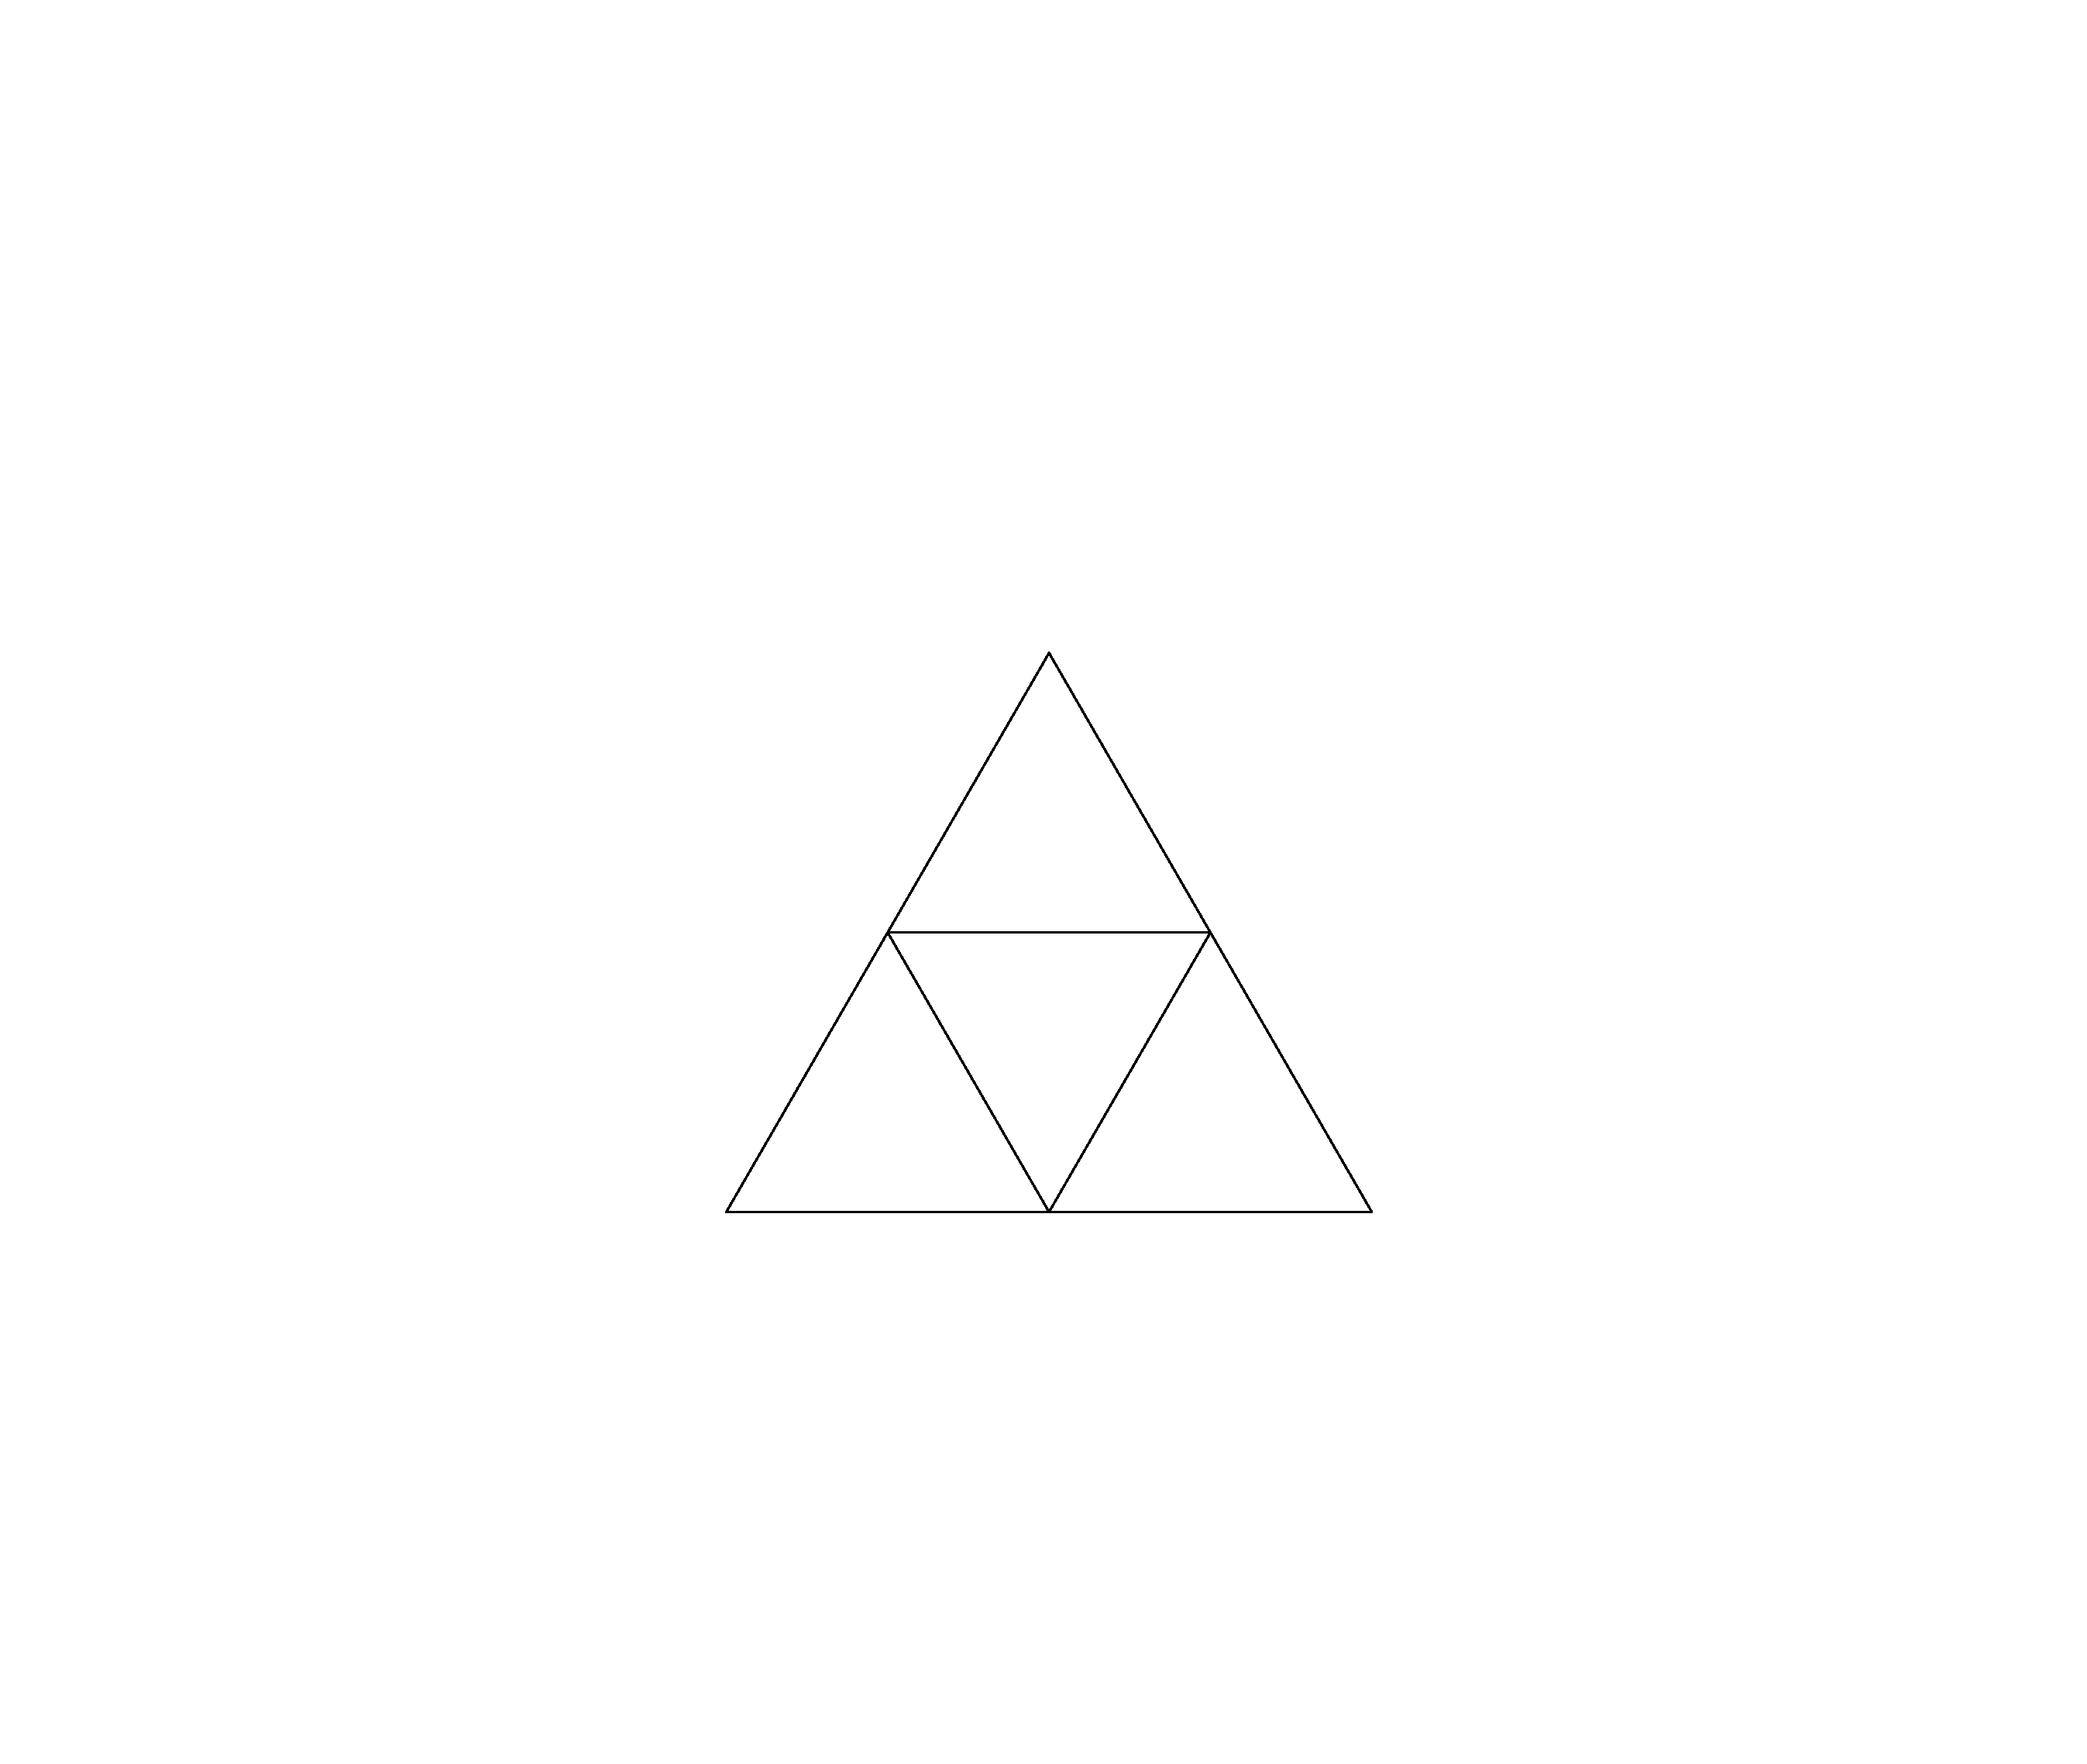
\includegraphics[trim=450 300 450 375,height=4cm]{2.eps}

\end{multicols}

\begin{multicols}{2}\raggedcolumns
\mysection{Exemple d'entrada 2}

\begin{verbatim}
100
5
\end{verbatim}


\columnbreak
\mysection{Exemple de sortida 2}

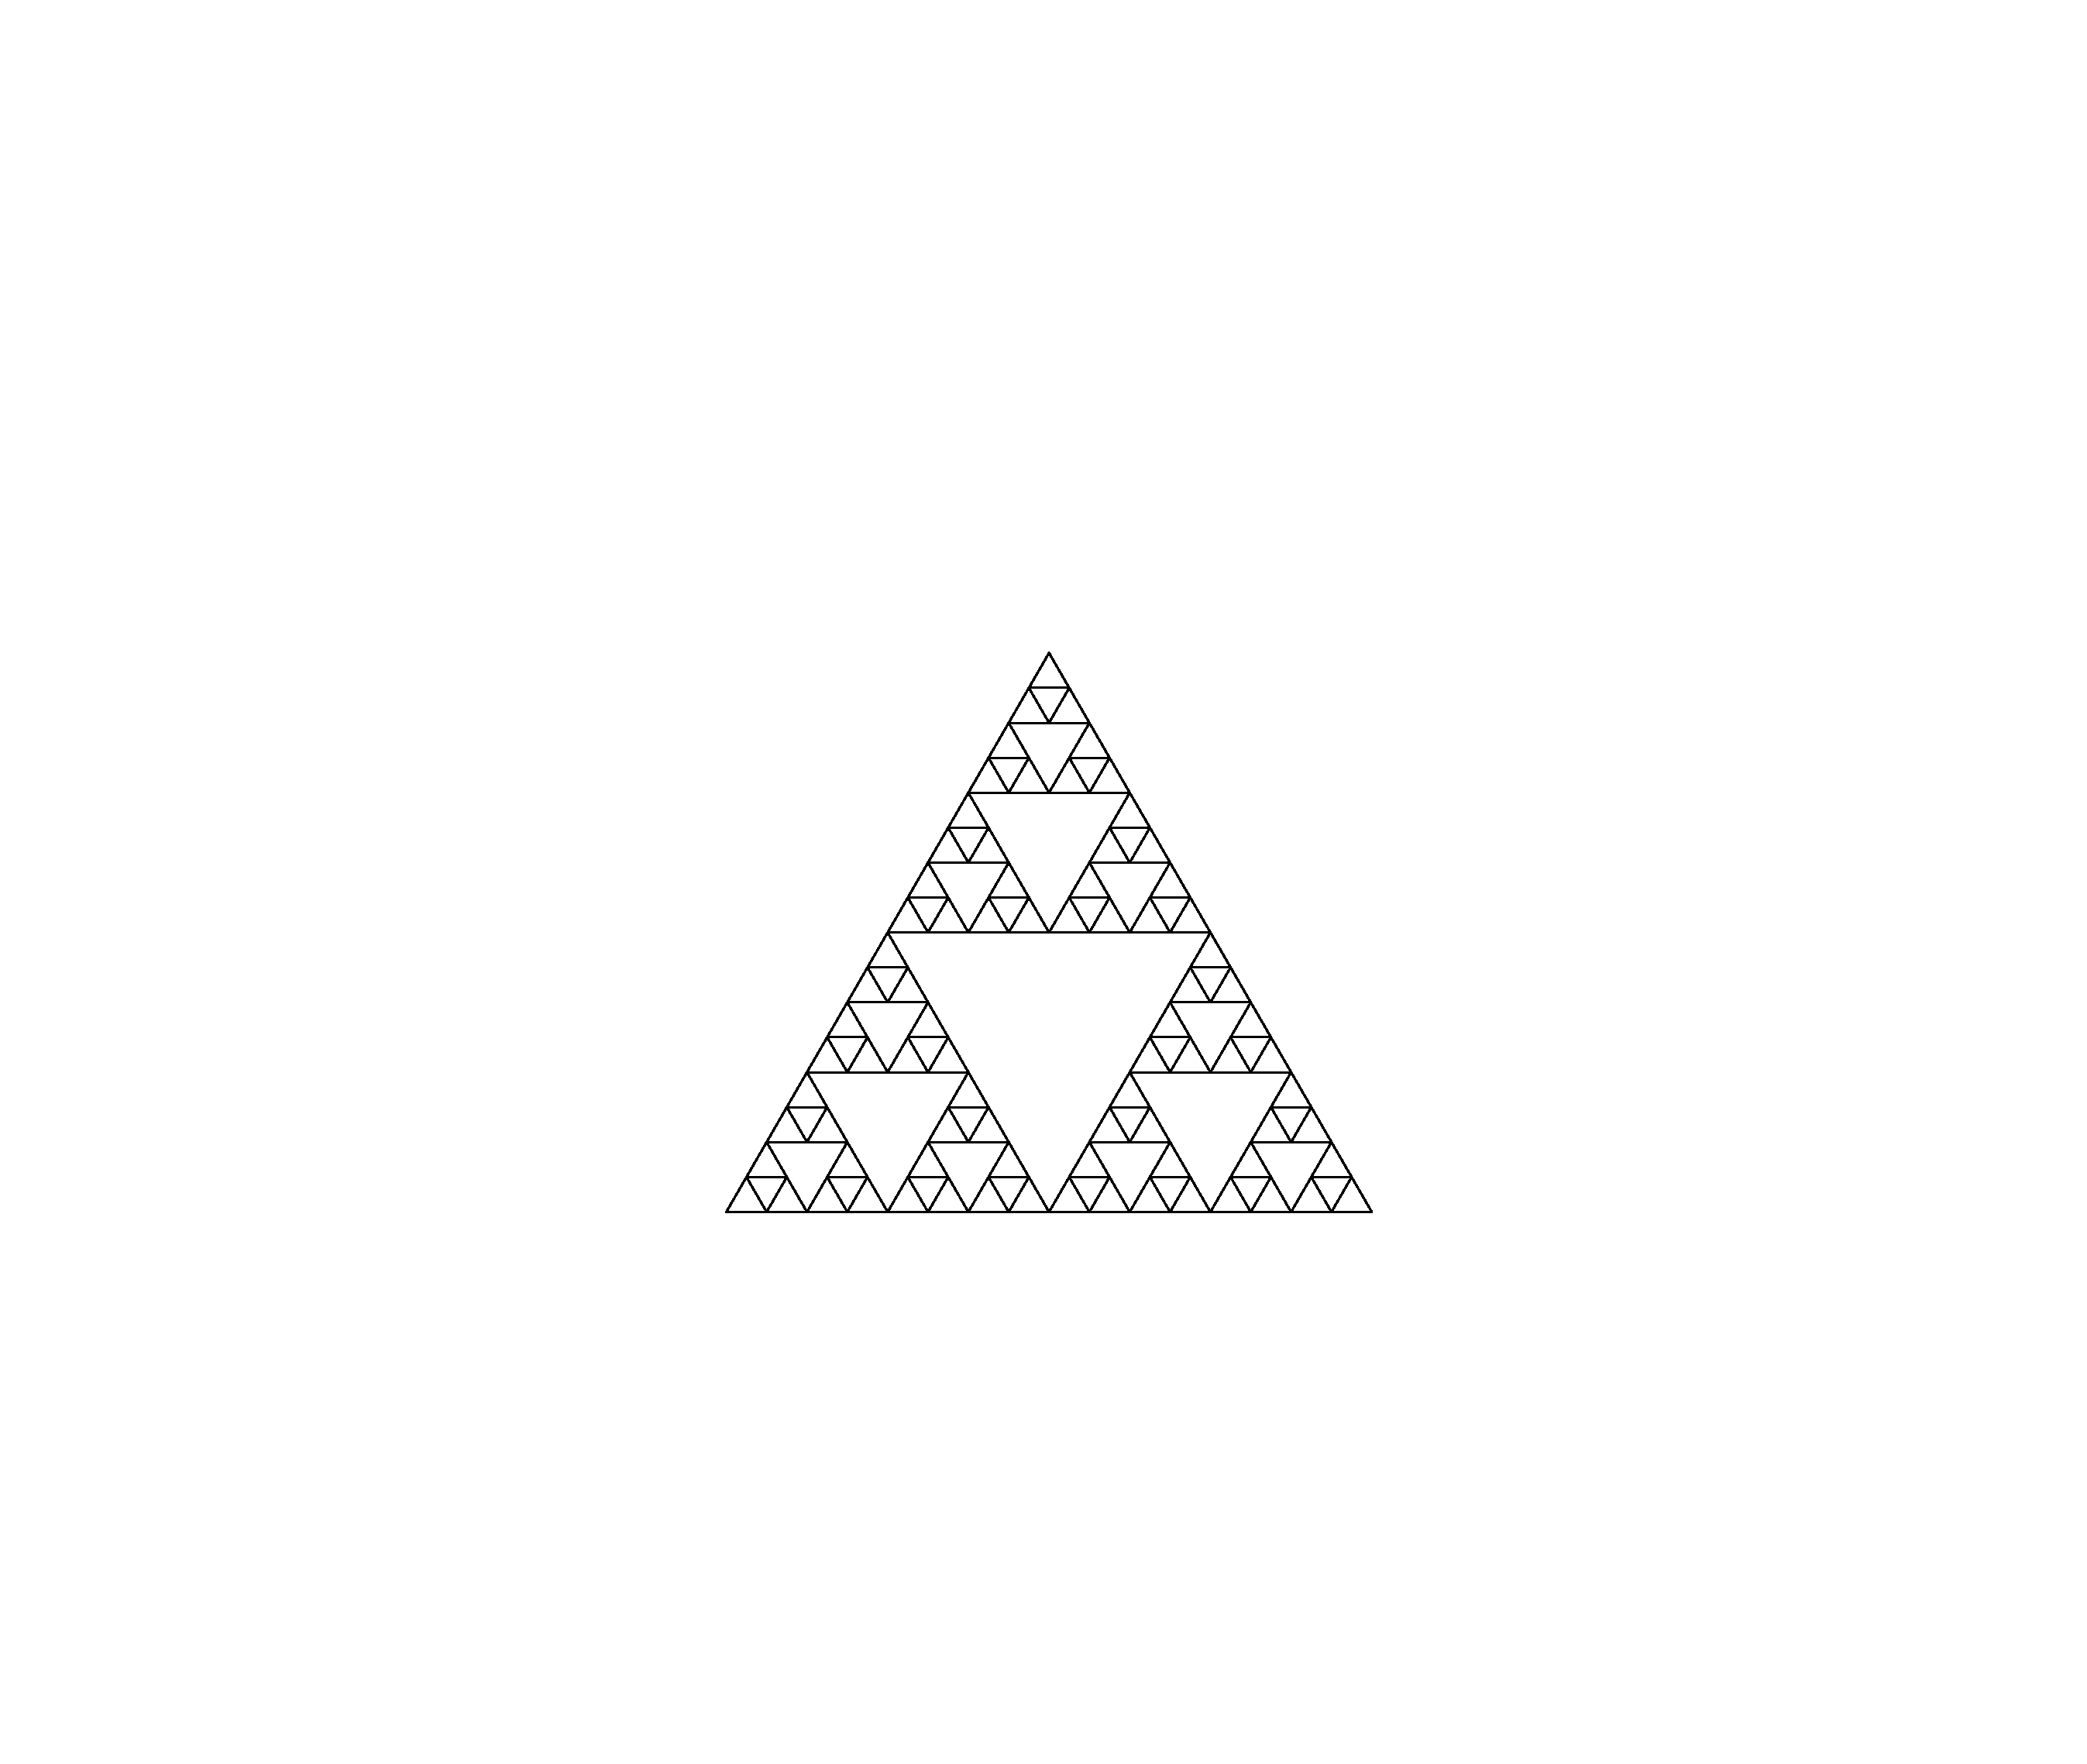
\includegraphics[trim=450 300 450 375,height=4cm]{5.eps}


\end{multicols}


\mysection{Recordatori}

Recordeu que Python ofereix un mòdul \texttt{turtle} que permet pintar images
amb una tortuga que es desplaça. Les úniques operacions que us calen són
\texttt{turtle.forward(m)} que avança la tortuga \texttt{m} unitats,
\texttt{turtle.backward(m)} que recula la tortuga \texttt{m} unitats,
\texttt{turtle.right(a)} que gira la tortuga \texttt{a} graus a la dreta i
\texttt{turtle.left(a)} que gira la tortuga \texttt{a} graus a l'esquerra.
També, podeu usar \texttt{turtle.speed(0)} per accelerar la tortuga.
Per exemple, aquest programa pinta un avorrit triangle:

\begin{small}
\begin{verbatim}
import turtle
import yogi

def triangle(m):
    for i in range(3):
        turtle.forward(m)
        turtle.left(120)

turtle.speed(0)
m = yogi.read(float)
triangle(m)
\end{verbatim}
\end{small}

\mysection{Observacions}

\begin{itemize}

\item Aquest problema no té jocs de proves al Jutge. Per tant, qualsevol solució serà
acceptada: semàfor verd! Això no vol dir que sigui bona ni dolenta, el vostre
professor ho corregirà.

\item
Perquè una solució sigui correcta no cal que cada segment es dibuixi
una sola vegada.

\end{itemize}
